\chapter{Implementation}

\section{Data Model} % (fold)

\subsection{Database Schema} % (fold)
\label{sub:database_schema}

	In this project, we used three table for storing all the information from users. As Figure~\ref{fig:data-schema} shows, Events is the main table in the app. It provides fields ``address'', ``comment'', ``creationDate'', ``latitude'', ``longitude'', ``locationName'', ``rate'', ``thumbnail'', ``photoBlob'' and ``tags''. ``address'' field is used when user didn't find their ``locationName'' in location List fetching from Foursquare API v2. ``Latitude'' and ``longitude'' is used for adding annotations in Map View. A 80*80 resolution thumbnail is stored for each event in order to accelerate loading in food list table. \\ 
	
	``photoBlob'' has one to one relationship with ``photo'' in PhotoBlob table. Using a separate table should also help speeding up when we don't need to load photo while we still need to get the meta data of the event. \\
	
	Field ``tags'' has many to many relationship with ``photos'' in Tag table since one photo can labeled with many tags and one tag can relate to many photos.  
	
\label{sec:data_model}
\begin{figure}
	\centering
    \SetFigLayout{1}{1}
    {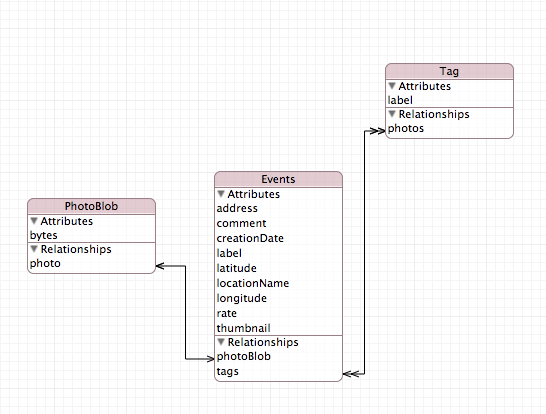
\includegraphics[%
    width=\figwidth, totalheight=\figheight, keepaspectratio]{./screenshots/database_schema.png}}
    \caption{Database Schema}
	\label{data-schema}
\end{figure}

% subsection database_schema (end)

\subsection{Settings Property List} % (fold)
\label{sub:settings_list}

	When developing iOS, we can also use another way to store data we need. Property List is used to store all information related to the app itself. For instance, using Property List to store App Display Name, App Version are commonly used in all apps for iPhone. \\
	
	``Fancy Foodie'' uses release number as main version string and git hash tag of the release as build string, so ``1.0 (build 98a9e84)'' is shown in Figure~\ref{fig:settings} which means that the main version number is 1.0 and build hash tag is 98a9e84. \\
	 
	 This app also use property list to store whether we need to save photo to album locally. If this option is enabled, the app will create a album  named ``Fancy Foodie Photos'' and put photos in this album as shown in Figure~\ref{fig:album}.
	 
 	 
% subsection settings_list (end)
% section data_model (end)
\newpage

\section{Workflow} % (fold)
\label{sec:work_overflow}

\subsection{Insert New Event} % (fold)
\label{sub:insert_new_event}

% subsection insert_new_event (end)

\subsection{Update Event} % (fold)
\label{sub:update_event}

% subsection update_event (end)

\subsection{Delete Event} % (fold)
\label{sub:delete_event}

% subsection delete_event (end)

\subsection{Searching Logic} % (fold)
\label{sub:searching_logic}

% subsection searching_logic (end)
\newpage
% section work_overflow (end)
\section{User Interface Design} % (fold)
\label{sec:user_interface_design}

\subsection{Home Tab} % (fold)
\label{sub:tabs}


\begin{figure}
    \centering
    \SetFigLayout{3}{3}
    \subfigure[Guide View]{
\includegraphics[width=\figwidth, totalheight=\figheight, keepaspectratio]{./screenshots/home.png}} \hfill
    \subfigure[Pick Action]{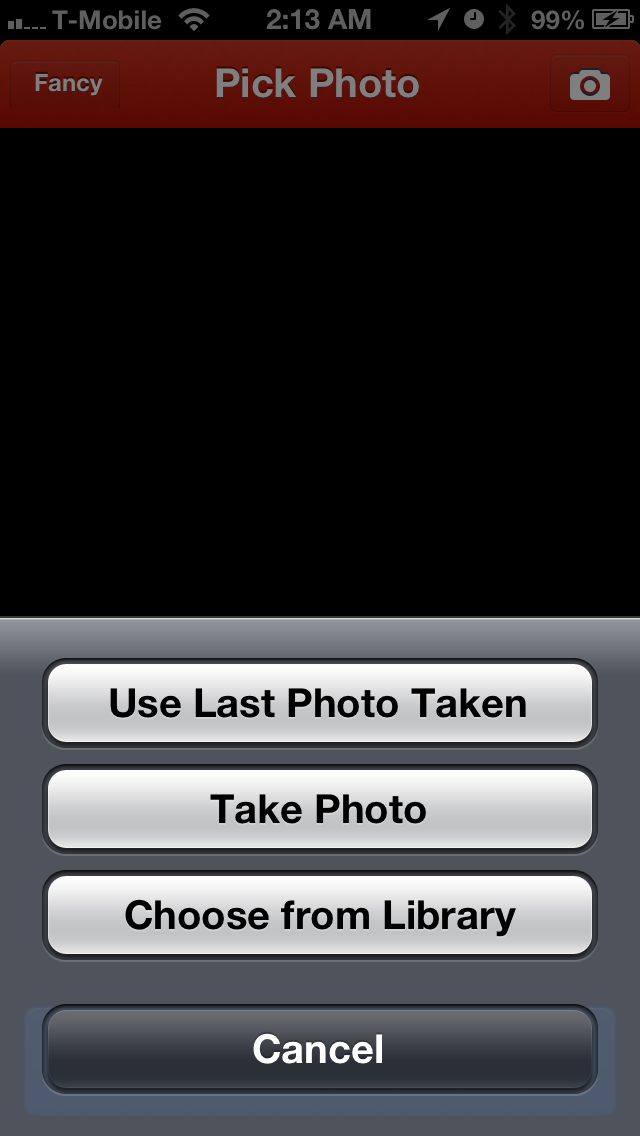
\includegraphics[width=\figwidth, totalheight=\figheight, keepaspectratio]{./screenshots/home-pickaction.png}} \hfill
	\subfigure[Move and Scale]{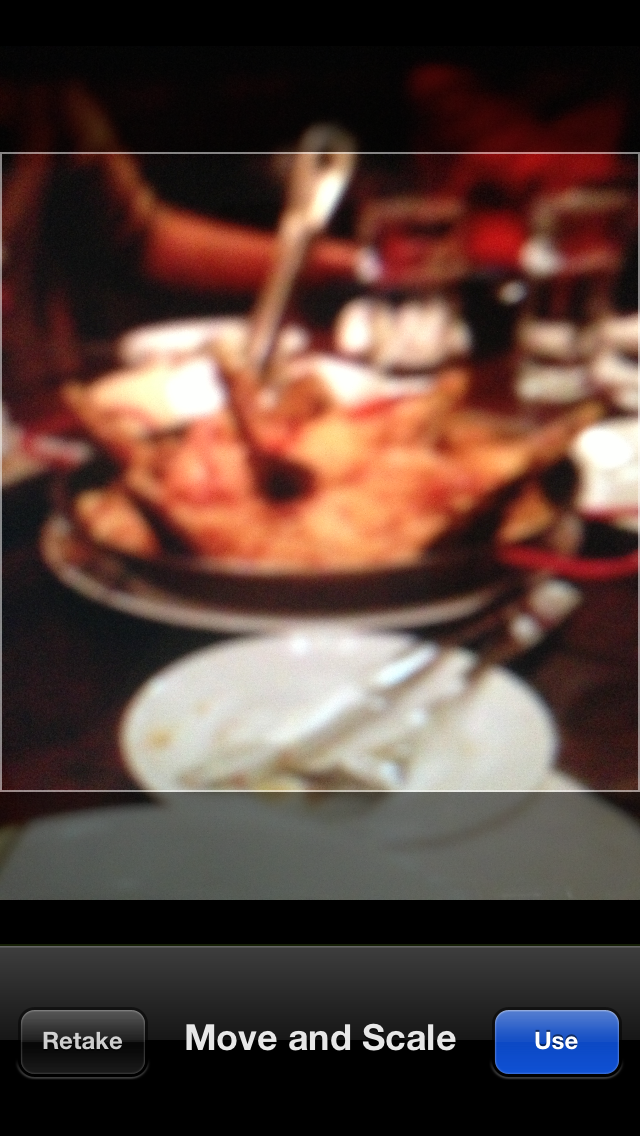
\includegraphics[width=\figwidth, totalheight=\figheight, keepaspectratio]{./screenshots/home-moveandscale.png}} \\ \hfill
    \subfigure[After Picking]{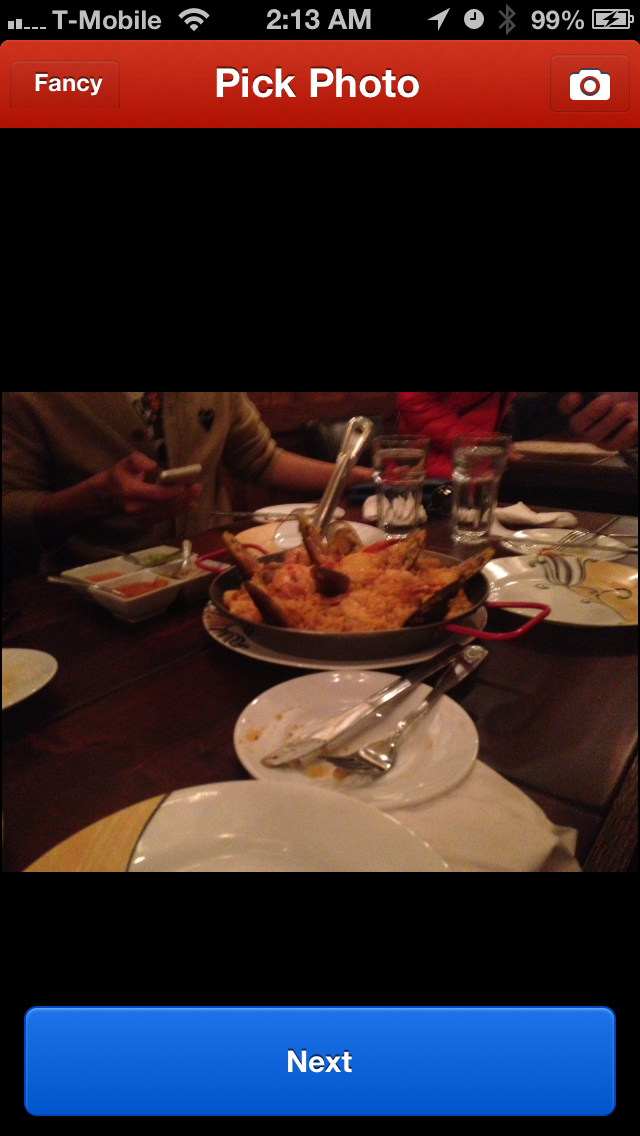
\includegraphics[width=\figwidth, totalheight=\figheight, keepaspectratio]{./screenshots/home-didpick.png}} \hfill
	\subfigure[Event Form]{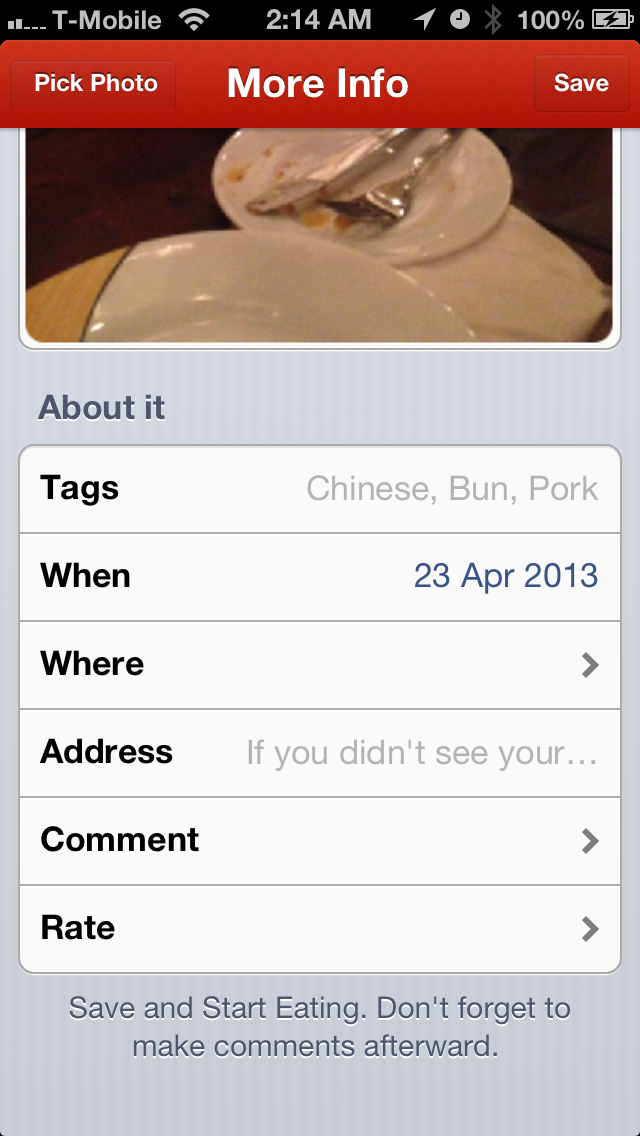
\includegraphics[width=\figwidth, totalheight=\figheight, keepaspectratio]{./screenshots/home-moreinfocontd.png}}   \hfill
    \subfigure[Date Picker]{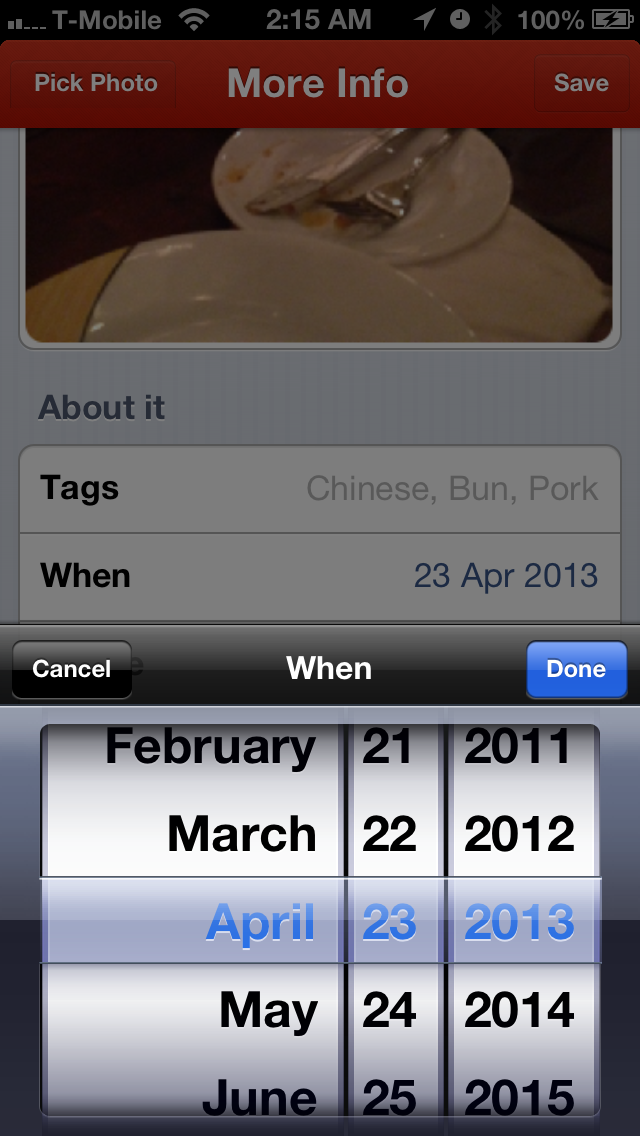
\includegraphics[width=\figwidth, totalheight=\figheight, keepaspectratio]{./screenshots/home-when.png}} \\ \hfill
    \subfigure[Location Picker]{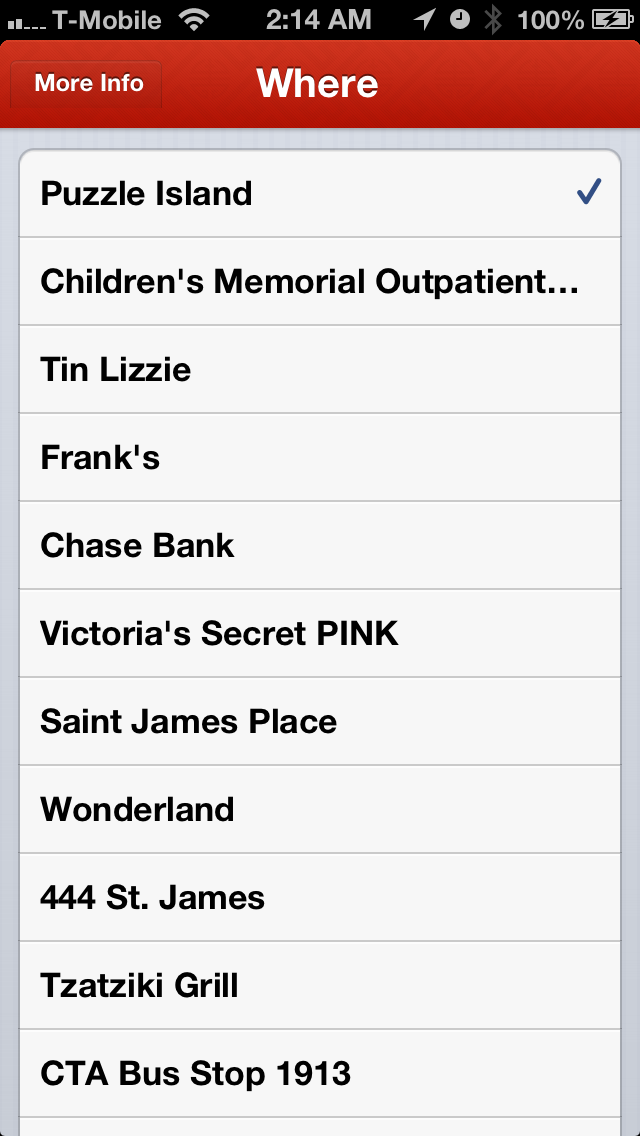
\includegraphics[width=\figwidth, totalheight=\figheight, keepaspectratio]{./screenshots/home-where.png}} \hfill
	\subfigure[Comment Editor]{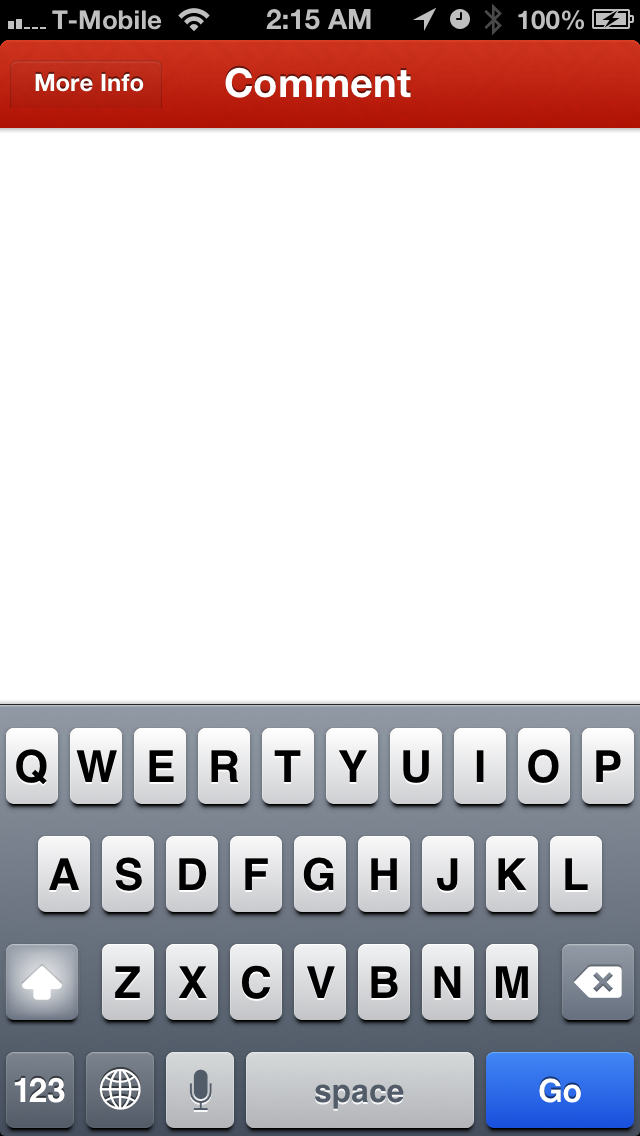
\includegraphics[width=\figwidth, totalheight=\figheight, keepaspectratio]{./screenshots/home-comment.png}}  \hfill
	\subfigure[Rate Picker]{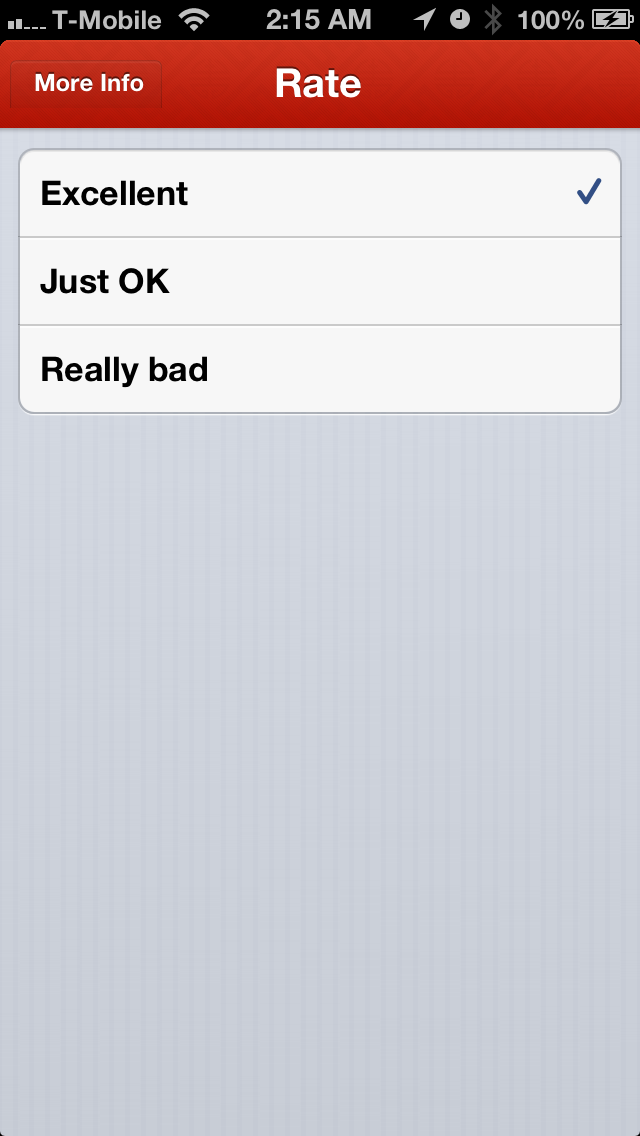
\includegraphics[width=\figwidth, totalheight=\figheight, keepaspectratio]{./screenshots/home-rate.png}} \hfill
	\caption{Home Tab View}
	\label{fig:hometab}
\end{figure}



% subsection tabs (end)

\subsection{Foodie List Tab} % (fold)
\label{sub:foodie_list_tab}

\begin{figure}
    \centering
    \SetFigLayout{2}{2}
    \subfigure[Foodie List]{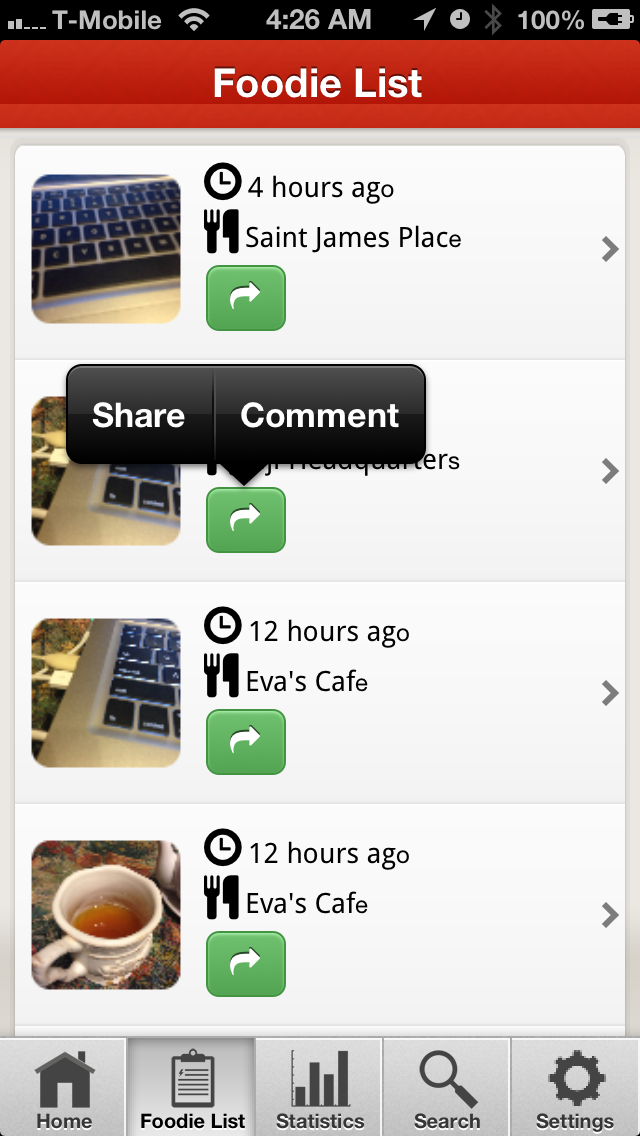
\includegraphics[width=\figwidth, totalheight=\figheight, keepaspectratio]{./screenshots/foodielist.png}} \hfill
	\subfigure[Sharing]{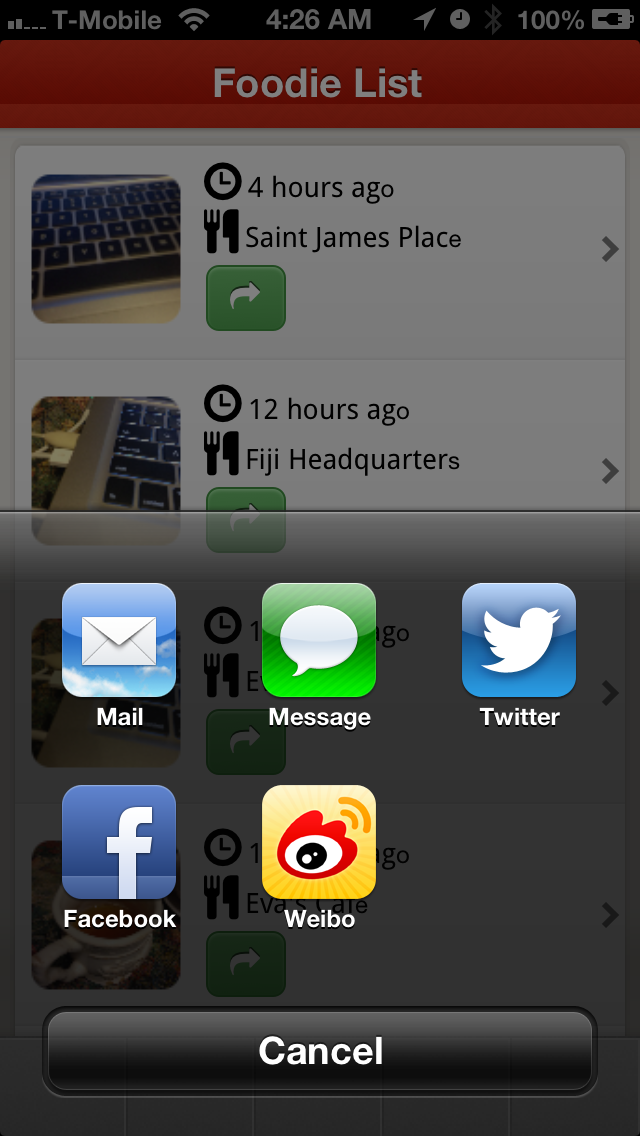
\includegraphics[width=\figwidth, totalheight=\figheight, keepaspectratio]{./screenshots/foodielist-share.png}} \hfill \\
	\subfigure[Detail View]{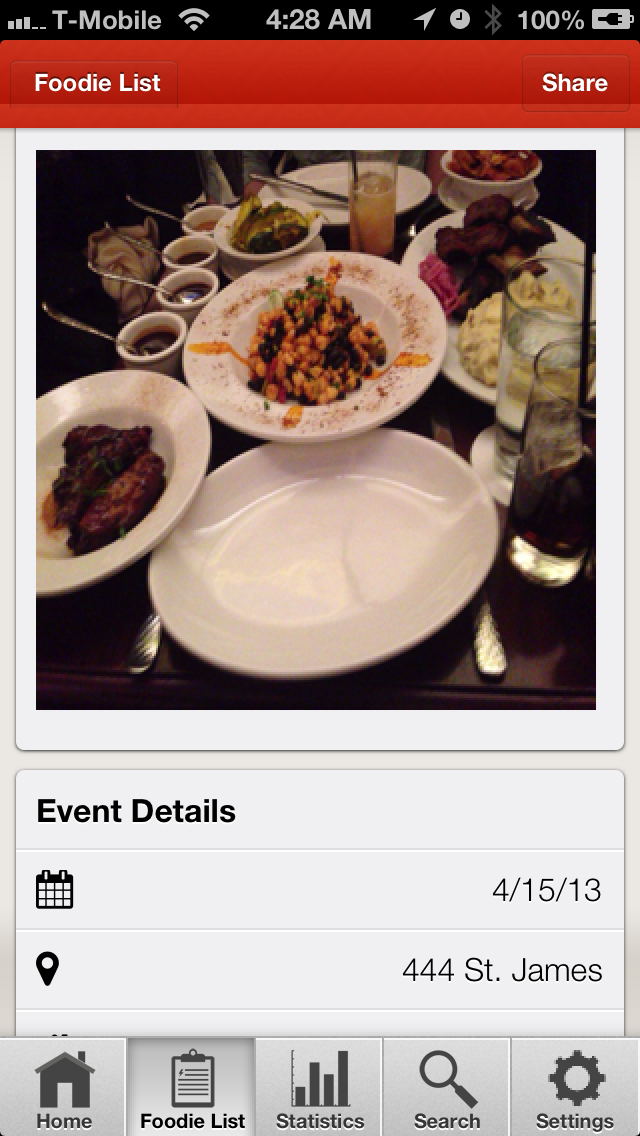
\includegraphics[width=\figwidth, totalheight=\figheight, keepaspectratio]{./screenshots/foodielist-detail.png}} \hfill
	\subfigure[Detail View Cont'd]{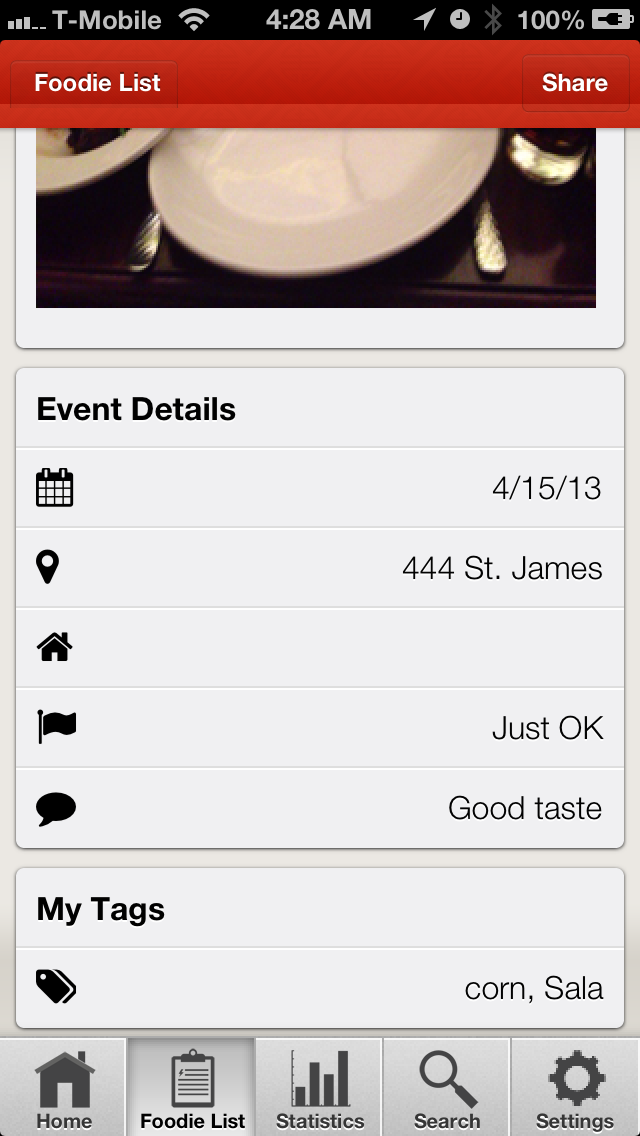
\includegraphics[width=\figwidth, totalheight=\figheight, keepaspectratio]{./screenshots/home-form-continued.png}} \hfill
	\caption{Foodie List Tab View}
	\label{fig:foodielisttab}
\end{figure}




% subsection foodie_list_tab (end)

\subsection{Stats Tab} % (fold)
\label{sub:stats_tab}

\begin{figure}
	\centering
    \SetFigLayout{1}{1}
    {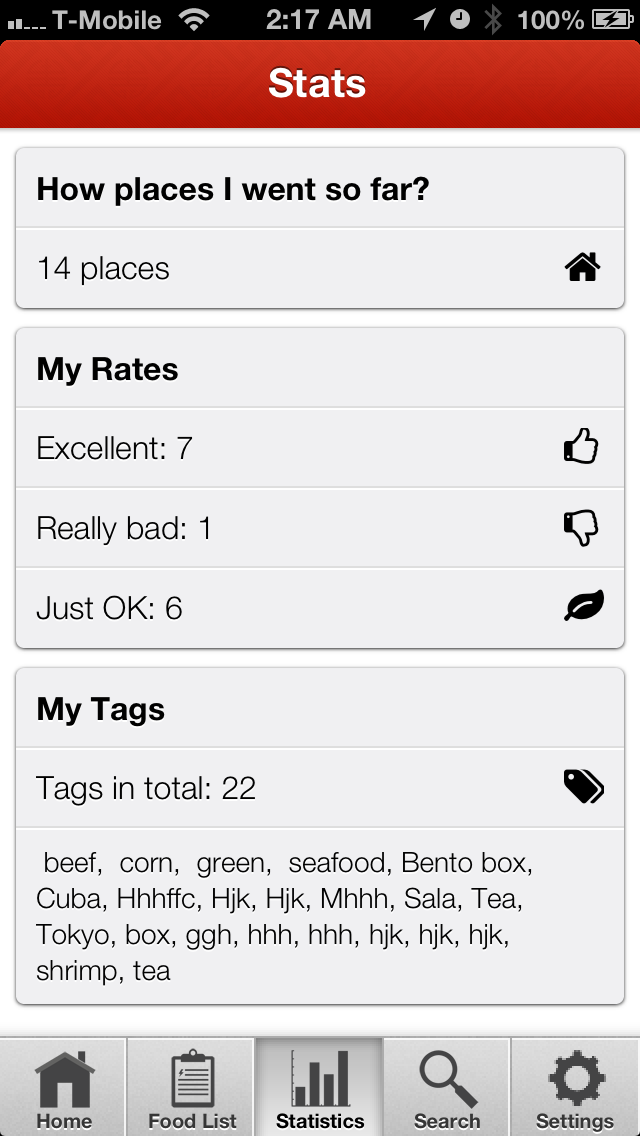
\includegraphics[%
    width=\figwidth, totalheight=\figheight, keepaspectratio]{./screenshots/stats.png}}
    \caption{Statistics Tab View}
\end{figure}

% subsection stats_tab (end)
\subsection{Map Tab} % (fold)
\label{sub:map_tab}

\begin{figure}
	\centering
    \SetFigLayout{1}{1}
    {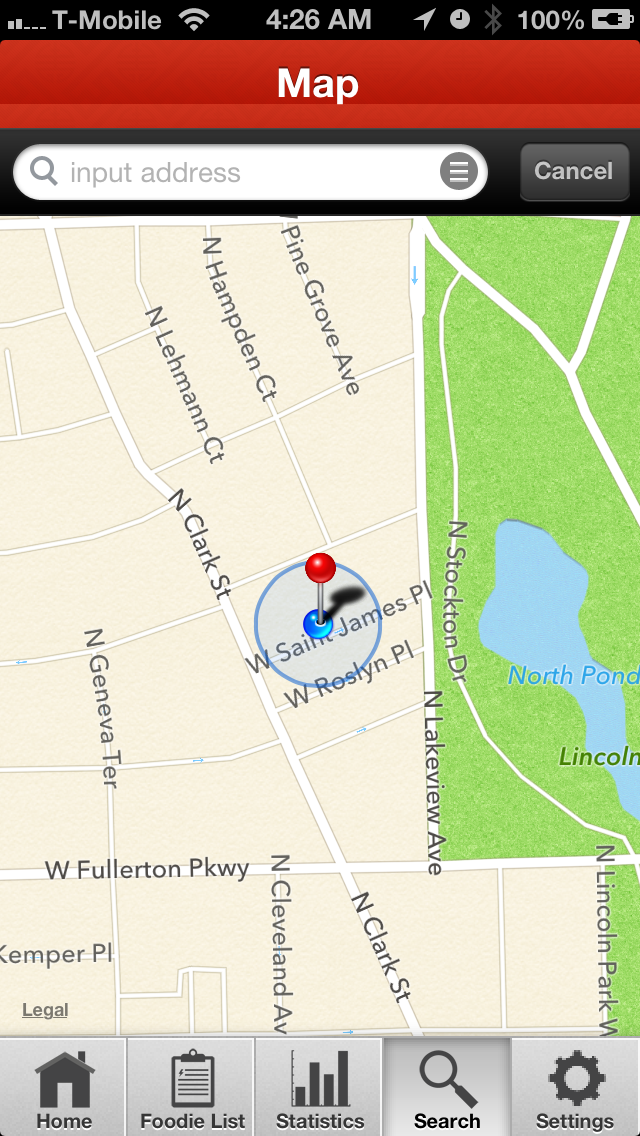
\includegraphics[%
    width=\figwidth, totalheight=\figheight, keepaspectratio]{./screenshots/map.png}}
    \caption{Map Tab View}
\end{figure}

% subsection map_tab (end)

\subsection{Setting Tab} % (fold)
\label{sub:setting_tab}

\begin{figure}
	\centering
    \SetFigLayout{1}{1}
    {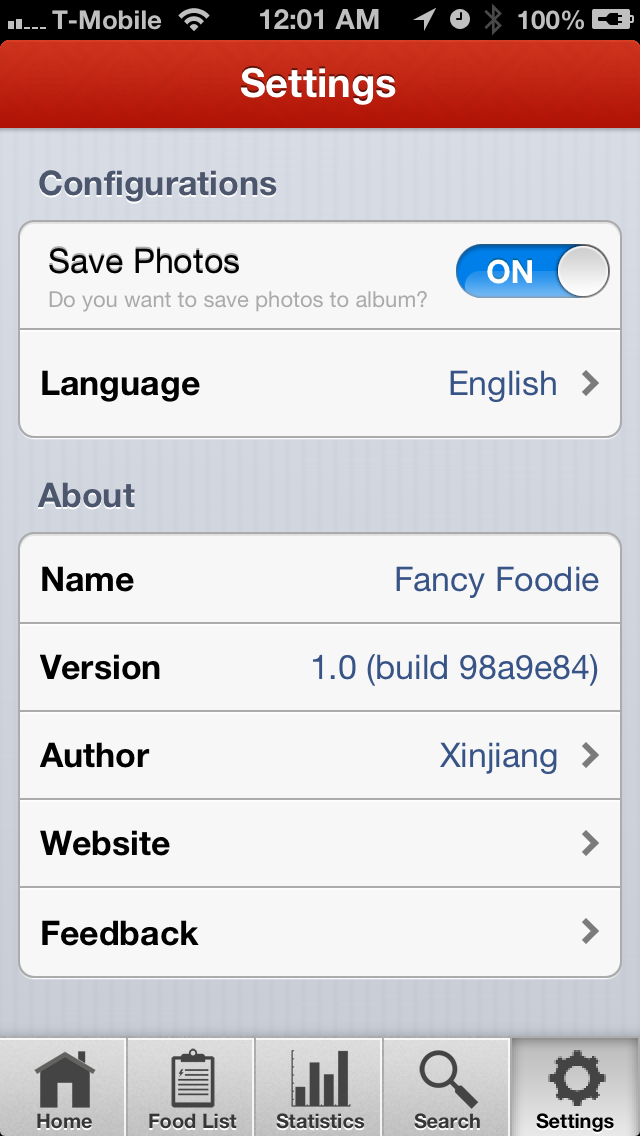
\includegraphics[%
    width=\figwidth, totalheight=\figheight, keepaspectratio]{./screenshots/settings.png}}
    \caption{Setting Tab View}
	\label{settings}
\end{figure}
\begin{figure}
	\centering
    \SetFigLayout{1}{1}
    {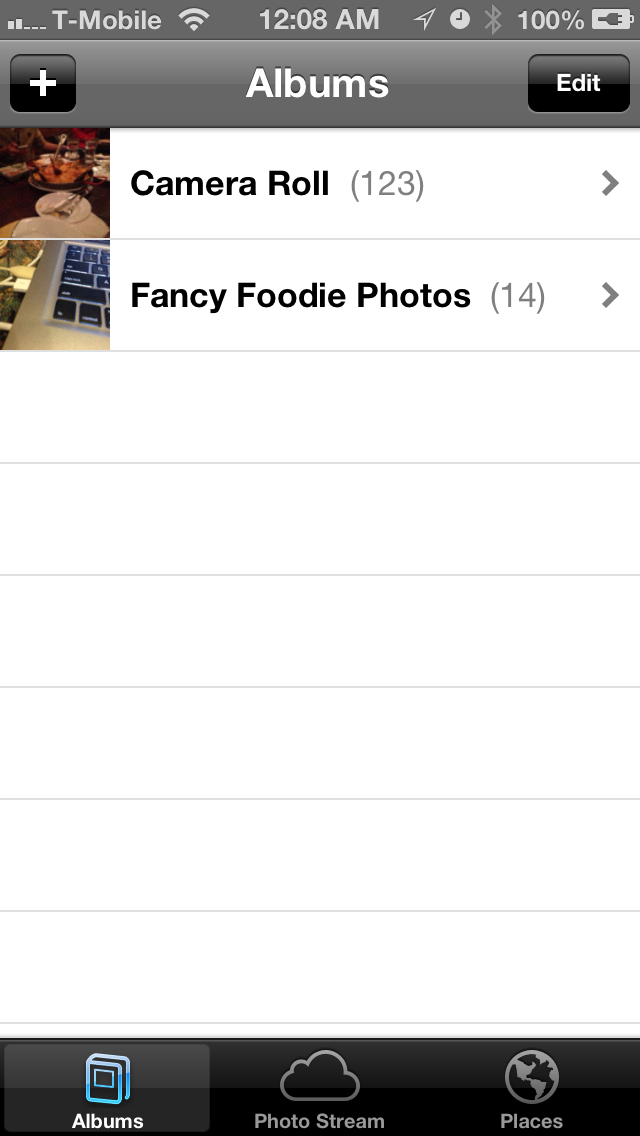
\includegraphics[%
    width=\figwidth, totalheight=\figheight, keepaspectratio]{./screenshots/settings-album.png}}
    \caption{Album View}
	\label{album}
\end{figure}
% subsection setting_tab (end)
% section user_interface_design (end)
